\let\lesson\undefined
\newcommand{\lesson}{\phantomlesson{Bài 3.}}


\setcounter{section}{2}
\section{Bài tập trắc nghiệm}
\begin{enumerate}[label=\bfseries Câu \arabic*:]
\item \mkstar{1}\\
{Chọn đáp án có từ /cụm từ thích hợp để hoàn thành bảng sau:
	\begin{center}
		\begin{tabular}{|c|c|c|}
			\hline
			\thead{Đơn vị} & \thead{Kí hiệu} & \thead{Đại lượng }\\
			\hline
			kelvin & (1) & (2)\\
			\hline
			ampe & $\si{\ampere}$ & (3)\\
			\hline
			candela & $\si{\candela}$ & (4)\\
			\hline
		\end{tabular}
	\end{center}
\begin{mcq}
	\item (1) $\si{\kelvin}$; (2) Khối lượng; (3) Cường độ dòng điện; (4) Lượng chất.
	\item (1) $\si{\kelvin}$; (2) Nhiệt độ; (3) Cường độ dòng điện; (4) Cường độ ánh sáng.
	\item (1) $\si{\kelvin}$; (2) Nhiệt độ; (3) Cường độ dòng điện; (4) Lượng chất.
	\item (1) $\si{\kelvin}$; (2) Khối lượng; (3) Cường độ dòng điện; (4) Cường độ ánh sáng.
\end{mcq}
}
\hideall{
\textbf{Đáp án: B.}
}

\item \mkstar{1}\\
{Đơn vị nào sau đây không thuộc thứ nguyên $L$ [Chiều dài]?
	\begin{mcq}(4)
		\item Dặm.
		\item Hải lí.
		\item Năm ánh sáng.
		\item Năm.
	\end{mcq}
}
\hideall{
\textbf{Đáp án: D.}
}


\item \mkstar{1}\\
{Chọn đáp án có từ/cụm từ thích hợp để hoàn thành các câu sau:
	\begin{itemize}
		\item[-] Các số hạng trong phép cộng (hoặc trừ) phải có cùng (1) \dots và nên chuyển về cùng (2) \dots.
		\item[-] (3) \dots của một biểu thức vật lí phải có cùng thứ nguyên.
	\end{itemize}
\begin{mcq}
	\item (1) đơn vị; (2) thứ nguyên; (3)  Đại lượng.
	\item (1) thứ nguyên; (2) đại lượng; (3) Hai vế.
	\item (1) đơn vị; (2) đại lượng; (3) Hai vế.
	\item (1) thứ nguyên; (2) đơn vị; (3) Hai vế.
\end{mcq}
}
\hideall{
\textbf{Đáp án: D.}
}

\item \mkstar{2}\\
{Trong các phép đo dưới đây, đâu là phép đo trực tiếp?
	\begin{enumerate}[label=(\arabic*)]
		\item Dùng thước đo chiều cao.
		\item Dùng cân đo cân nặng.
		\item Dùng cân và ca đong đo khối lượng riêng của nước.
		\item Dùng đồng hồ và cột cây số đo tốc độ của người lái xe.
	\end{enumerate}
\begin{mcq}(4)
	\item (1), (2).
	\item (1), (2), (4).
	\item (2), (3), (4).
	\item (2), (4).
\end{mcq}
}
\hideall{
\textbf{Đáp án: A.}
}

\item \mkstar{2}\\
{Đáp án nào sau đây có 1 đơn vị cơ bản và 1 đơn vị dẫn xuất?
	\begin{mcq}(2)
		\item Mét, kilogram.
		\item Newton, mol.
		\item Pascal, joule.
		\item Candela, kelvin.
	\end{mcq}
}
\hideall{
\textbf{Đáp án: B.}
}

\item \mkstar{2}\\
{Giá trị nào sau dây có 2 chữ số có nghĩa (CSCN)?
	\begin{mcq}(4)
		\item $\SI{201}{\meter}$.
		\item $\SI{0.02}{\meter}$.
		\item $\SI{20}{\meter}$.
		\item $\SI{210}{\meter}$.
	\end{mcq}

}
\hideall{
\textbf{Đáp án: D.}
}

\item \mkstar{3}\\
{Một bánh xe có bán kính $R=\xsi{10\pm0,5}{\centi\meter}$. Sai số tương đối của chu vi bánh xe là
	\begin{mcq}(4)
		\item $\SI{0.05}{\percent}$.
		\item $\SI{5}{\percent}$.
		\item $\SI{10}{\percent}$.
		\item $\SI{25}{\percent}$.
	\end{mcq}
}
\hideall{
\textbf{Đáp án: B.}
}
\end{enumerate}
\section{Bài tập tự luận}
\begin{enumerate}[label=\bfseries Bài \arabic*:]
	\item \mkstar{2}
	
	
	{
		Em hãy lập phương án đo tốc độ chuyển động của ô tô đồ chơi, chỉ dùng thước và đồng hồ bấm giây để trả lời các câu hỏi sau:
		\begin{enumerate}[label=\alph*)]
			\item Để đo tốc độ chuyển động của chiếc xe, cần đo những đại lượng nào?
			\item Xác định tốc độ chuyển động của xe theo công thức nào?
			\item Phép đo nào là phép đo trực tiếp? Tại sao?
			\item Phép đo nào là phép đo gián tiếp? Tại sao?
		\end{enumerate}
		
	}
	
	\hideall
	{	
		\begin{enumerate}[label=\alph*)]
			\item Để đo tốc độ chuyển động của chiếc xe, cần đo những đại lượng: đo quãng đường xe di chuyển được và thời gian xe di chuyển.
			\item Xác định tốc độ chuyển động của xe theo công thức:
			
			$$v = \dfrac{s}{t}.$$
			
			\item Phép đo quãng đường và thời gian là phép đo trực tiếp. Vì ta thực hiện động tác trực tiếp lên các dụng cụ thí nghiệm.
			\item Phép đo xác đinh vận tốc là phép đo gián tiếp. Vì phép đo này có được cần phải thông qua hai phép đo kia.
		\end{enumerate}
	}

\item \mkstar{2}\\
{Hình \ref{fig:3P-1} thể hiện nhiệt kế đo nhiệt độ $t_1$ $\left(\si{\degree C}\right)$ và $t_2$ $\left(\si{\degree C}\right)$ của một dung dịch trước và sau khi đun. Hãy xác định và ghi kết quả độ tăng nhiệt độ $t$ của dung dịch này.
	\begin{center}
		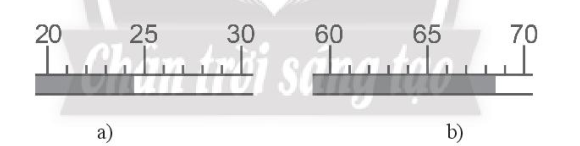
\includegraphics[width=0.4\linewidth]{../figs/VN10-2022-PH-TP003-P-1}
		\captionof{figure}{Nhiệt kế: \textit{a) trước; b) sau khi đun dung dịch}}
		\label{fig:3P-1}
	\end{center}
}
\hideall{
$$t=\xsi{44,0\pm1,0}{\degree C}.$$
}

\item \mkstar{2}\\
{Hãy xác định số CSCN của các số sau đây: $123,45$; $1,990$; $3,110\cdot 10^{-9}$; $1907,21$; $0,002099$; $12768000$. 

}
\hideall{
$123,45$ - 5 CSCN; $1,990$ - 4 CSCN; $3,110\cdot10^{-9}$ - 4 CSCN; $1907,21$ - 6 CSCN; $0,002099$ - 4 CSCN; $12768000$ - 5 CSCN.
}
	
	\item \mkstar{2}\\
	{Một viên bị hình cầu có bán kính $r$ đang chuyển động với tốc độ $v$ trong dầu. Viên bị chịu tác dụng của lực cản có độ lớn được cho bởi biểu thức $F=c\cdot r\cdot v$, trong đó $c$ là một hằng số. Xác định đơn vị của $c$ theo đơn vị của lực, chiều dài và thời gian trong hệ SI.
}
\hideall{
Đơn vị của $c$ là: $\si{\newton\cdot\meter^{-2}\cdot\second}$.
}
	
	\item \mkstar{2}\\
	{Một vật có khối lượng $m$ và thể tích $V$, có khối lượng riêng $\rho$ được xác định bằng công thức $\rho =\dfrac{m}{V}$. Biết sai số tương đối của phép đo $m$ và $V$ lần lượt là $\SI{12}{\percent}$ và $\SI{15}{\percent}$. Hãy xác định sai số tương đối của phép đo $\rho$.
	
}
\hideall{
$$\delta \rho=\SI{17}{\percent}.$$
}
	
	\item \mkstar{2}\\
	{Một học sinh muốn xác định gia tốc rơi tự do $g$ bằng cách thả một quả bóng từ độ cao $h$ và dùng đồng hồ để bấm thời gian rơi $t$ của quả bóng. Sau đó, thông qua quá trình tìm hiểu, bạn sử dụng công thức $h=\dfrac{1}{2}g\cdot t^2$ để xác định $g$. Hãy nêu ít nhất 2 giải pháp giúp bạn học sinh đó giảm sai số trong quá trình thực nghiệm để thu được kết quả chính xác nhất.
	
}
\hideall{
Một số giải pháp phù hợp: hạn chế sự tác động của lực cản không khí, thả rơi quả bóng ở nhiều độ cao khác nhau, sử dụng đồng hồ có độ nhạy cao, thao tác bấm đồng hồ dứt khoát.
}

\item \mkstar{2}


{
	\begin{center}
		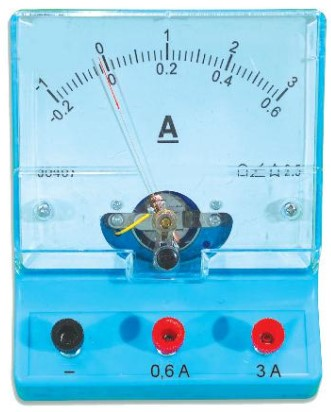
\includegraphics[scale=0.6]{../figs/VN10-2022-PH-TP003-6.jpg}
	\end{center}
	\begin{enumerate}[label=\alph*)]
		\item Giới hạn đo của ampe kế là bao nhiêu?
		\item Nếu sử dụng ampe kế để đo dòng điện vượt quá giới hạn đo thì có thể gây ra nguy cơ gì?
	\end{enumerate}
}

\hideall
{	
	\begin{enumerate}[label=\alph*)]
		\item Giới hạn đo của ampe kế ở hình là $\SI{3}{A}$.
		\item Nếu sử dụng ampe kế để đo dòng điện vượt quá giới hạn đo thì có thể làm cho ampe kế bị hư hỏng.
	\end{enumerate}
}



\item \mkstar{3}\\
{Hãy xác định số đo chiều dài của cây bút chì trong các trường hợp dưới đây:
	\begin{center}
		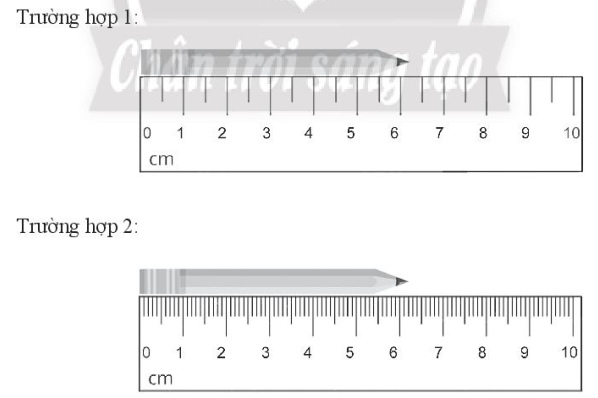
\includegraphics[width=0.6\linewidth]{../figs/VN10-2022-PH-TP003-P-2}
	\end{center}

}
\hideall{
\begin{itemize}
	\item Trường hợp 1: $\ell=\xsi{6,0\pm0,3}{\centi\meter}$.
	\item Trường hợp 2: $\ell=\xsi{6,20\pm0,05}{\centi\meter}$.
\end{itemize}
}
	
	\item \mkstar{3}
	
	{
		Đo chiều dày của một cuốn sách, được kết quả: $\SI{2,3}{cm}$; $\SI{2,4}{cm}$; $\SI{2,5}{cm}$; $\SI{2,4}{cm}$. Tính giá trị trung bình chiều dày cuốn sách. Sai số tuyệt đối trung bình của phép đo này là bao nhiêu?
	}
	
	\hideall{
		
		Ta có: 
		
		$$\overline{A} = \dfrac{A_1 + A_2 +...+ A_n}{n} =\SI{2,4}{cm}.$$
		
		Vậy trung bình chiều dày cuốn sách là $\SI{2,4}{cm}.$
		
		$$\Delta A_1 = |\overline{A} - A_1| = \text{0,1}.$$
		
		$$\Delta A_2 = |\overline{A} - A_2| = 0.$$
		
		$$\Delta A_3 = |\overline{A} - A_3| = \text{0,1}.$$
		
		$$\Delta A_4 = |\overline{A} - A_4| = 0.$$
		
		Ta có:
		
		$$\Delta \overline{A} = \dfrac{\Delta A_1 + \Delta A_2 +\Delta A_3+ \Delta A_4}{4} =\SI{0,05}{cm}.$$
		
		Vậy sai số tuyệt đối trung bình là $\SI{0,05}{cm}.$
	}
	
	\item \mkstar{3}
	
	{
		
		Bảng ghi thời gian một vật rơi giữa hai điểm cố định:
		
		\begin{center}
			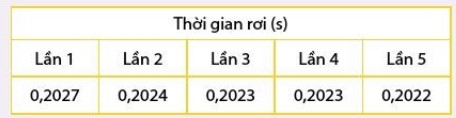
\includegraphics[scale=1]{../figs/VN10-2022-PH-TP003-1.jpg}
		\end{center}
		\begin{enumerate}[label=\alph*)]
			\item Tính giá trị trung bình của thời gian rơi.
			\item Tìm sai số tuyệt đối trung bình.
		\end{enumerate}
	}
	
	\hideall{
		
		\begin{enumerate}[label=\alph*)]
			\item Giá trị trung bình của thời gian rơi là:
			
			$$\dfrac{\text{0,2027} + \text{0,2024}+ \text{0,2023}+ \text{0,2023}+ \text{0,2022}}{5} \approx \text{0,2024}$$
			
			\item Sai số tuyệt đối:
			
			$$A_1= |\text{0,2024} - \text{0,2027}| = \text{0,0003}.$$
			
			$$A_2= |\text{0,2024} - \text{0,2024}| = \text{0,0000}.$$
			
			$$A_3= |\text{0,2024} - \text{0,2023}| = \text{0,0001}.$$
			
			$$A_4= |\text{0,2024} - \text{0,2023}| = \text{0,0001}.$$
			
			$$A_5= |\text{0,2024} - \text{0,2022}| = \text{0,0002}.$$
			
			Sai số tuyệt đối trung bình là: 
			
			$$\dfrac{\text{0,0003} + \text{0,0000} + \text{0,0001} + \text{0,0001}  + \text{0,0002}}{5} = \text{0,00014}.$$	\end{enumerate}
		
	}

	
	
	

	\item \mkstar{4}
	
	
	{
		Dùng thước kẹp có ĐCNN $\SI{0,1}{mm}$ để đo 5 lần đường kính $d$ và chiều cao $h$ của một trụ thép, cho kết quả như trong bảng sau:
		
		\begin{center}
			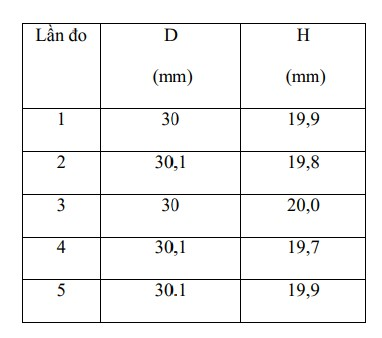
\includegraphics[scale=1]{../figs/VN10-2022-PH-TP003-8.jpg}
		\end{center}
		
		Hãy cho biết kết quả phép đo $d, h$ và tính thể tích trụ thép.
	}
	
	\hideall
	{	
		Phép đo $d, h$ là phép đo trực tiếp, giá trị
		trung bình và sai số ngẫu nhiên tính trong
		bảng sau
		
		\begin{center}
			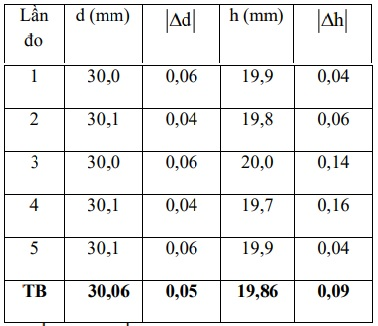
\includegraphics[scale=1]{../figs/VN10-2022-PH-TP003-9.jpg}
		\end{center}
		
		Sai số dụng cụ bằng $\SI{0,1}{mm}$. Vậy:
		
		Sai số phép đo đường kính trụ là:
		
		$$\Delta d = \text{0,05} + \text{0,1} =\SI{0,15}{mm}.$$
		
		Sai số phép đo chiều cao trụ là:
		
		$$\Delta h = \text{0,09} + \text{0,1} =\SI{0,19}{mm}.$$
		
		Kết quả: 
		
		$$d = \text{30,06} \pm \text{0,15}\ (\text{mm}).$$
		
		$$h = \text{19,86} \pm \text{0,19}\ (\text{mm}).$$
		
		Thể tích trung bình của khối trụ:
		
		$$\overline{V}  = \dfrac{\pi \bar{d}^2 \bar{h}}{4} =\SI{14100}{mm}^3.$$
		
		Sai số tỉ đối:
		
		$$\dfrac{\Delta V}{\overline V} = 2 \dfrac{\overline{\Delta d}}{\overline d} + \dfrac{\overline {\Delta h}}{\overline{h}} + \dfrac{\Delta \pi}{\pi} = \text{0,02} = 2\%.$$
		
		Sai số tuyệt đối:
		
		$$\Delta V = \overline{V} \delta V = \SI{282}{mm}^3.$$
		
		Suy ra:
		
		$$V = 14100 \pm 280 \ \text{mm}^3.$$
		
		
	}
	
\end{enumerate}